\chapter{Sensing Platform} \label{sensing_platform}


        

%%%%%%%%%%%%%%%%%
% \subsection{Livox LiDAR} \label{sensors_LiDAR}

% The Minion platform features six \ac{LiDAR} units providing both omnidirectional environmental awareness and forward-facing high-density perception.
% The \ac{LiDAR} suite comprises three Velodyne HDL-32E units and three Livox Horizon units.

% The three Velodyne HDL-32E mechanically rotating 360-degree \ac{LiDAR} sensors are positioned to provide complete omnidirectional point cloud coverage.
% One unit is positioned at aft-center, with the other two placed at approximately one-third intervals around the vessel at forward-port and forward-starboard locations to achieve a full 360-degree \ac{FOV} coverage.

% The three Livox Horizon solid-state forward-scanning \ac{LiDAR} sensors provide high-density returns within a 165-degree forward \ac{FOV} matching the camera array coverage.
% These sensors were selected specifically for \ac{LiDAR}-camera fusion research based on superior point cloud density within the camera \ac{FOV} and a non-repetitive scan pattern that enhances coverage through temporal aggregation \cite{thompson2023}.

% While 360-degree coverage provides comprehensive spatial awareness, it presents challenges for camera-\ac{LiDAR} fusion.
% First, sparse azimuthal sampling occurs because on a stationary or slow-moving platform, the 32 lasers strike identical positions on every rotation, yielding no increase in sampling density over time.
% Second, inefficient \ac{FOV} utilization results from distributing returns across 360 degrees, such that only a fraction falls within the forward-facing camera view.
% These limitations motivated the selection of an alternative \ac{LiDAR} technology optimized for forward-facing perception with temporal aggregation.

% The Livox Horizon employs a non-repetitive rosette scan pattern that progressively covers its \ac{FOV} over time rather than repeatedly sampling identical locations.
% The sensor features an 81.7-degree × 25.1-degree (horizontal × vertical) \ac{FOV}, substantially wider in azimuth than the 65-degree cameras.
% Three Livox units deployed together achieve a combined coverage of approximately 165 × 25.1 degrees, providing complete horizontal overlap with the camera array and covering approximately 77\% vertically \cite{thompson2023}.
% Table 3.2 presents the Livox Horizon specifications.

% \begin{table}[htpb]
% \centering
% \caption{LiDAR Specifications}
% \begin{tabular}{ll}
% \hline
% \multicolumn{2}{c}{Livox Horizon}\\
% \hline
% % \textbf{Parameter} & \textbf{Value} \\
% \hline
% Model & Livox Horizon \\
% Horizontal Field of View & 81.7 degree \\
% Vertical Field of View & 25.1 degree \\
% Range & 260 m @ 80\% reflectivity \\
% Point Rate (Single Return) & 240,000 pts/sec \\
% Point Rate (Dual Return) & 480,000 pts/sec \\
% Range Precision & ±2 cm \\
% Wavelength & 905 nm \\
% Scan Pattern & Non-repetitive rosette \\
% Interface & Ethernet \\
% Operating Frequency & 100 Hz \\
% \hline
% \end{tabular}
% \label{tab:livox_horizon_specs}
% \end{table}



% The non-repetitive scan pattern demonstrates particular advantage when aggregating multiple scans over time, accumulating points over an integration window to enhance spatial sampling.
% On a moving platform, motion compensation during the accumulation period becomes necessary.
% The \ac{LiDAR} aggregation approach, detailed in Chapter 5, employs the \ac{GPS}/\ac{IMU} to track platform pose over time.
% Each \ac{LiDAR} point is transformed from sensor coordinates to a world reference frame using the platform pose at that point's timestamp.
% All accumulated points are then transformed from world coordinates to the target camera image frame, enabling overlay of a dense point cloud on the image.
% A four-second integration period was selected based on empirical evaluation of the tradeoff between point cloud density and motion blur.
% Each camera image sampled at 1 Hz receives all \ac{LiDAR} points from the preceding four seconds, transformed to the image capture time.
% This approach provides the spatial resolution necessary for reliable detection while maintaining sufficient motion compensation accuracy for typical vessel speeds.

% The Livox Horizon sensors communicate via \ac{UDP} over Ethernet, transmitting point cloud data as binary messages at 100 Hz.
% Livox provides an open-source \ac{ROS} SDK that manages network communication, message parsing, and point cloud publication to \ac{ROS} topics.
% Integration of the Livox SDK into the Minion software required minimal effort, primarily involving network configuration and modification of \ac{ROS} launch files.
% The SDK operates on the Atlas PC, receiving \ac{UDP} messages from all three \ac{LiDAR} units simultaneously over the local network described in Section 3.1.2.3.

% Accurate fusion of data from multiple \ac{LiDAR} units requires precise knowledge of sensor geometric relationships.
% The Livox Horizon units feature onboard storage for extrinsic calibration parameters, enabling each sensor to transform its measurements to a common reference frame before transmission.
% The \ac{LiDAR}-to-\ac{LiDAR} extrinsic calibration presented in Section 3.2.1.3 determines the six-degree-of-freedom transformation (translation and rotation) relating each sensor's local coordinates to the designated primary sensor.
% These parameters are written to non-volatile memory on each Livox unit, configuring automatic application of the transformation such that all point clouds emerge in the center \ac{LiDAR}'s reference frame \cite{thompson2023}.
% This onboard configuration simplifies downstream processing by eliminating the need for software-based registration of the three point clouds.
% The unified cloud is subsequently related to camera coordinates through camera-to-\ac{LiDAR} extrinsic calibration described in Section 3.2.1.2.

% Temporal alignment of \ac{LiDAR} with camera images and \ac{GPS}/\ac{IMU} pose requires all \ac{LiDAR} points to possess timestamps referenced to a common global time base.
% The Livox Horizon supports IEEE 1588 Precision Time Protocol, providing sub-microsecond clock synchronization with a \ac{PTP} master on the network.
% In this configuration, the NVIDIA Jetson Xavier in the camera box functions as the \ac{PTP} master, synchronizing the three \ac{LiDAR} units.
% The Jetson itself synchronizes to \ac{GPS} time via the Network Time Protocol hierarchy detailed in Section 3.2.2.1.
% This cascaded synchronization ensures \ac{LiDAR} timestamps share the same \ac{GPS}-disciplined time reference as camera frames, enabling frame-accurate alignment for fusion.
% \ac{PTP} synchronization status is verified using the Livox Viewer software, which displays sync state and time source for each sensor.
% Proper \ac{PTP} lock is confirmed prior to data collection, ensuring timestamp accuracy.

% An advantageous characteristic of the 905 nm wavelength is its strong absorption by water.
% This results in minimal \ac{LiDAR} returns from water surfaces, contrasting with vision sensors that clearly image water texture and waves.
% Absence of water returns reduces point cloud clutter and simplifies object detection by eliminating the need to filter ground plane points for the water surface.
% Point cloud visualizations overlaid on camera images demonstrate this characteristic: dense \ac{LiDAR} coverage appears on vessels, buoys, and other solid objects, while water surfaces produce few or no returns.
% For grid-based clustering, this characteristic prevents false positives from wave crests or foam patterns.

% The Livox Horizon configuration provides several capabilities essential for comparing object detection performance.
% The system achieves 2.25× more points within the camera view compared to omnidirectional spinning sensors, while the non-repetitive scan pattern enhances sampling density through temporal aggregation.
% Per-point timestamps and \ac{GPS}/\ac{IMU} integration enable accurate aggregation during motion, while \ac{PTP} synchronization provides sub-microsecond timing accuracy relative to cameras and \ac{GPS}.
% Factory-configured multi-sensor calibration unifies point clouds from three sensors before transmission, and the 905 nm wavelength reduces maritime clutter by rejecting water returns.
% Combined with the software integration and synchronization infrastructure described in Section 3.2, this configuration enables rigorous \ac{LiDAR} detection evaluation and comparison with vision-based approaches in Chapters 5 and 6.

%%%%%%%%%%%%%%%%%%
\subsection{LiDAR Systems} \label{sensors_LiDAR}

The Minion platform features six \ac{LiDAR} units providing both omnidirectional environmental awareness and forward-facing high-density perception.
The \ac{LiDAR} suite comprises three Velodyne HDL-32E units and three Livox Horizon units.

The three Velodyne HDL-32E mechanically rotating 360-degree \ac{LiDAR} sensors are positioned at aft-center, with the other two placed at approximately one-third intervals around the vessel at forward-port and forward-starboard locations to achieve full 360-degree \ac{FOV} coverage.
These sensors provide the spatial awareness necessary for autonomous navigation and collision avoidance.

The three Livox Horizon forward-scanning \ac{LiDAR} sensors provide high-density returns within the camera's \ac{FOV} and serve as the primary \ac{LiDAR} sensors for this research.
While the Velodyne units provide adequate omnidirectional awareness for navigation, they present fundamental limitations for camera-\ac{LiDAR} fusion research.

% MOTIVATION - Why Livox over Velodyne
LiDAR sensors with fixed 360-degree scan patterns, such as the Velodyne HDL-32E, impose limitations on object-detection research.
Because the scan maintains a constant elevation and azimuth with each rotation, the sensor repeatedly samples the same positions, resulting in a sparse representation of objects with a low relative velocity to the sensor.
This parallels the resolution of optical cameras; lower density returns limit the ability to resolve features on small or distant objects, as the sparsity increases linearly with range.

The Livox Horizon addresses this limitation through a fundamentally different scan architecture.
Rather than repeatedly sampling fixed positions, the sensor employs a non-repetitive rosette scan pattern that progressively covers its \ac{FOV} over time, as visualized in Figure \ref{fig:livox_scan_pattern}.
This irregular sampling pattern produces substantially denser point cloud data, critical for the object detection methods described in Section \ref{gbcache}, and motivated their selection for the forward-scanning perception suite \cite{thompson2023}.


Each Livox Horizon sensor features an 81.7-degree (horizontal)\ac{FOV} and are mounted to provide more than 50\% overlap between units.
This configuration effectively doubles the number of returned points within the 65-degree \ac{FOV} of the primary forward camera and creates a system that is robust to individual sensor failure.
Table~\ref{tab:livox_horizon_specs} presents the Livox Horizon specifications.

\begin{table}[htpb]
\centering
\caption{LiDAR Specifications}
\begin{tabular}{ll}
\hline
\multicolumn{2}{c}{Livox Horizon}\\
\hline
% \textbf{Parameter} & \textbf{Value} \\
\hline
Model & Livox Horizon \\
Horizontal Field of View & 81.7 degree \\
Vertical Field of View & 25.1 degree \\
Range & 260 m @ 80\% reflectivity \\
Point Rate (Single Return) & 240,000 pts/sec \\
Point Rate (Dual Return) & 480,000 pts/sec \\
Range Precision & ±2 cm \\
Wavelength & 905 nm \\
Scan Pattern & Non-repetitive rosette \\
Interface & Ethernet \\
Operating Frequency & 100 Hz \\
\hline
\end{tabular}
\label{tab:livox_horizon_specs}
\end{table}

\begin{figure}[htbp]
\centering
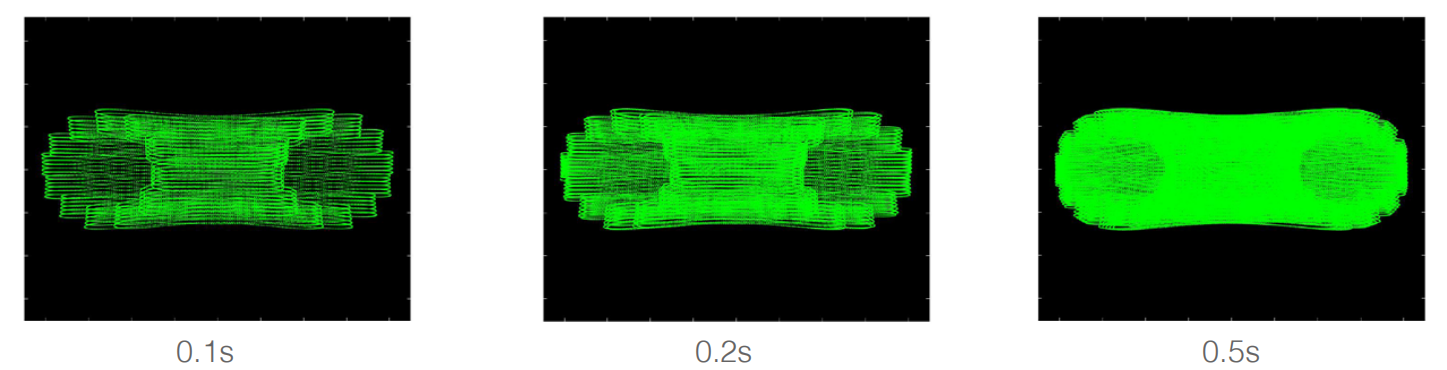
\includegraphics[width=0.8\textwidth]{Images/Livox_1.png}
\caption{Livox Horizon non-repetitive rosette scan pattern demonstrating point cloud density distribution from 0.1 to 0.5 seconds.}
\label{fig:livox_scan_pattern}
\end{figure}

% The sensor employs a two-dimensional scanning mechanism that traces a non-repetitive rosette pattern across the \ac{FOV}.
The sensor employs two orthogonal mirrors operating at slightly different frequencies to trace a complex Lissajous-like path that progressively fills the \ac{FOV} without repetition at a maximum rate of $480000$ points per second per device.
\textcolor{red}{cite Livox documentation?}.

The Livox Horizon sensors communicate via \ac{UDP} over Ethernet, transmitting point cloud data as binary messages at 100 Hz.
Each point consists of position coordinates (x, y, z), intensity, and timestamp, totaling 16 bytes per point.
At maximum point rate (480,000 pts/sec per sensor), three sensors generate approximately:

$$\text{Peak bandwidth} = 3 \times 480,000 \times 16 \text{ bytes/sec} \approx 23 \text{ Mbps}$$

In practice, the sensors are configured to suppress null returns (points beyond maximum range or with insufficient reflectivity), reducing actual network traffic below this theoretical maximum.
% The rosette pattern provides substantially higher spatial coverage compared to a spinning sensor's fixed ring geometry, particularly in the vertical dimension where traditional spinning sensors are limited to discrete horizontal rings.
% This density characteristic is critical for the grid-based clustering approach employed for \ac{LiDAR} object detection in Chapter 5.

The 905 nm near-infrared wavelength experiences strong absorption by water, resulting in minimal returns from water surfaces.
This characteristic benefits maritime object detection by reducing clutter from waves that would otherwise trigger false positives in clustering algorithms.
\textcolor{red}{Figure \#} demonstrates this effect: dense \ac{LiDAR} coverage appearing on vessels, buoys, and other solid objects, while water surfaces produce few or no returns.
\textcolor{red}{insert figure to compare Velodyne and Livox returns in situ.}

% Comparison of point cloud density within the camera \ac{FOV} quantifies the Livox advantage over traditional spinning sensors.
% A Velodyne HDL-32E in dual-return mode produces approximately 1.4 million points per second distributed across the full 360-degree plane.
% The camera \ac{FOV} encompasses approximately 165 degrees, yielding an effective point rate in the region of interest of:

% $$\text{Effective HDL-32E rate} = 1.4 \times 10^6 \times \frac{165°}{360°} \approx 641,000 \text{ pts/sec}$$

% Three Livox Horizon units in dual-return mode together produce:

% $$\text{Combined Livox rate} = 3 \times 480,000 = 1.44 \times 10^6 \text{ pts/sec}$$

% This represents a 2.25× increase in point returns within the camera view, excluding additional benefits from superior vertical sampling achieved through the non-repetitive pattern compared to fixed 32-ring geometry \cite{thompson2023}.



% Accurate fusion of data from multiple \ac{LiDAR} units requires precise knowledge of sensor geometric relationships.
The Livox Horizon units feature onboard storage for extrinsic calibration parameters, enabling each sensor to transform its measurements to a common reference frame before transmission.
These parameters are written to non-volatile memory on each Livox unit and applied before data transmission so that all LiDAR returns are received in the center \ac{LiDAR}'s reference frame, reducing the necessary calculation further down the data pipeline.
\textcolor{red}{cite Livox documentation?}.
% enhancing their real-time operational advantage by reducing additional computation later in the pipeline.
The calibration methodology to determine these extrinsic values is detailed in Section~\ref{lidar_extrinsic}.


%%%%%%%%%%%%%%%%%%
% \subsection{LWIR Thermal Cameras} \label{sensors_LWIR}
% Two Teledyne Calibir 640 \ac{LWIR} thermal cameras extend perception to night and low-light conditions. 
% While limited to 640×480 resolution due to bolometer technology, they provide a combined 165-degree forward \ac{FOV} when paired, ensuring redundancy with the
% visible and \ac{HDR} cameras.
% \textcolor{red}{Possibly remove this subsection?}





\subsubsection{HDR Selection}

The FLIR Blackfly S 4K cameras satisfy geometric and resolution requirements, but their limited dynamic range makes them prone to over-exposure and loss of highlight detail in high-contrast maritime conditions. 
They support an effective dynamic range of 69.4~dB, which corresponds to a span of just a few thousand-to-one between the darkest detectable signal and the brightest non-saturating signal. 
As a result, the cameras are prone to over-exposure in high-brightness maritime conditions, particularly when imaging reflective water surfaces or bright sky backgrounds, leading to loss of highlight detail and reduced contrast. 

In contrast, the IMX490 \ac{HDR} camera combines a comparable \ac{FOV} with substantially greater dynamic range, enabling detail preservation across bright and shaded regions within the same frame.  
For these reasons, the \ac{HDR} camera was designated as the primary forward-facing visual spectrum sensor for \ac{LiDAR}-camera fusion research.  
 
As a result, the cameras are prone to over-exposure in high-brightness maritime conditions, particularly when imaging reflective water surfaces or bright sky backgrounds, leading to loss of highlight detail and reduced contrast.  



        




\subsection{Sensor Transforms}
The multi-sensor system aboard the WAM-V requires rigorous coordinate frame transformations to fuse data from heterogeneous sensors into a unified representation. Each sensor operates in its native coordinate frame, necessitating extrinsic calibration to establish spatial relationships between sensors and the vessel's body frame.

The fundamental transformation between coordinate frames is expressed as:
\begin{equation}
^Bp =\; ^B_AR \; ^Ap + ^B_A T
\end{equation}
where points in reference frame $A$ ($^Ap$) are transformed into reference frame $B$ ($^Bp$) through a rotation matrix $^B_AR$ and translation vector $^B_A T$.

% \subsubsection{Coordinate Frame Definitions}
The selected sensors employ multiple coordinate frames, each with distinct conventions:

% \textbf{Inertial Frame (Map):} 
The global reference frame follows the North-East-Down (NED) convention, where the x-axis points north, y-axis points east, and z-axis points downward toward the earth's center. This right-handed frame provides a consistent world reference for navigation and localization.

% \textbf{LiDAR Frame:} 
The Livox Horizon sensors capture point cloud data in the Forward-Left-Up (FLU) convention, where x-axis points forward along the sensor's optical axis, y-axis points left, and z-axis points upward. Each of the three LiDAR units maintains this local frame relative to its mounting position.

% \textbf{GPS Frame:} 
The GPS receiver outputs position data in geodetic coordinates (latitude, longitude, altitude), which are converted to Cartesian coordinates in the FLU body frame using the vessel heading from the inertial measurement unit (IMU). This transformation accounts for the spherical earth geometry and local tangent plane approximation.

% \textbf{Camera Frame:} 
The Leopard Imaging camera operates in a standard image plane coordinate system where the u-axis (horizontal) points right, v-axis (vertical) points down, and the optical axis extends forward along the camera's line of sight. Image coordinates require both extrinsic transforms to the body frame and intrinsic camera calibration for 3D reconstruction.

The sensor-to-body and body-to-inertial transformations are all handled through the \Ac{ROS} robot-localization package onboard the \Acp{USV} main computer, Atlas.
%%%%%%%%%%%%%%%%%%%%%%%%%%%%%%
\begin{figure}[htbp]
\centering
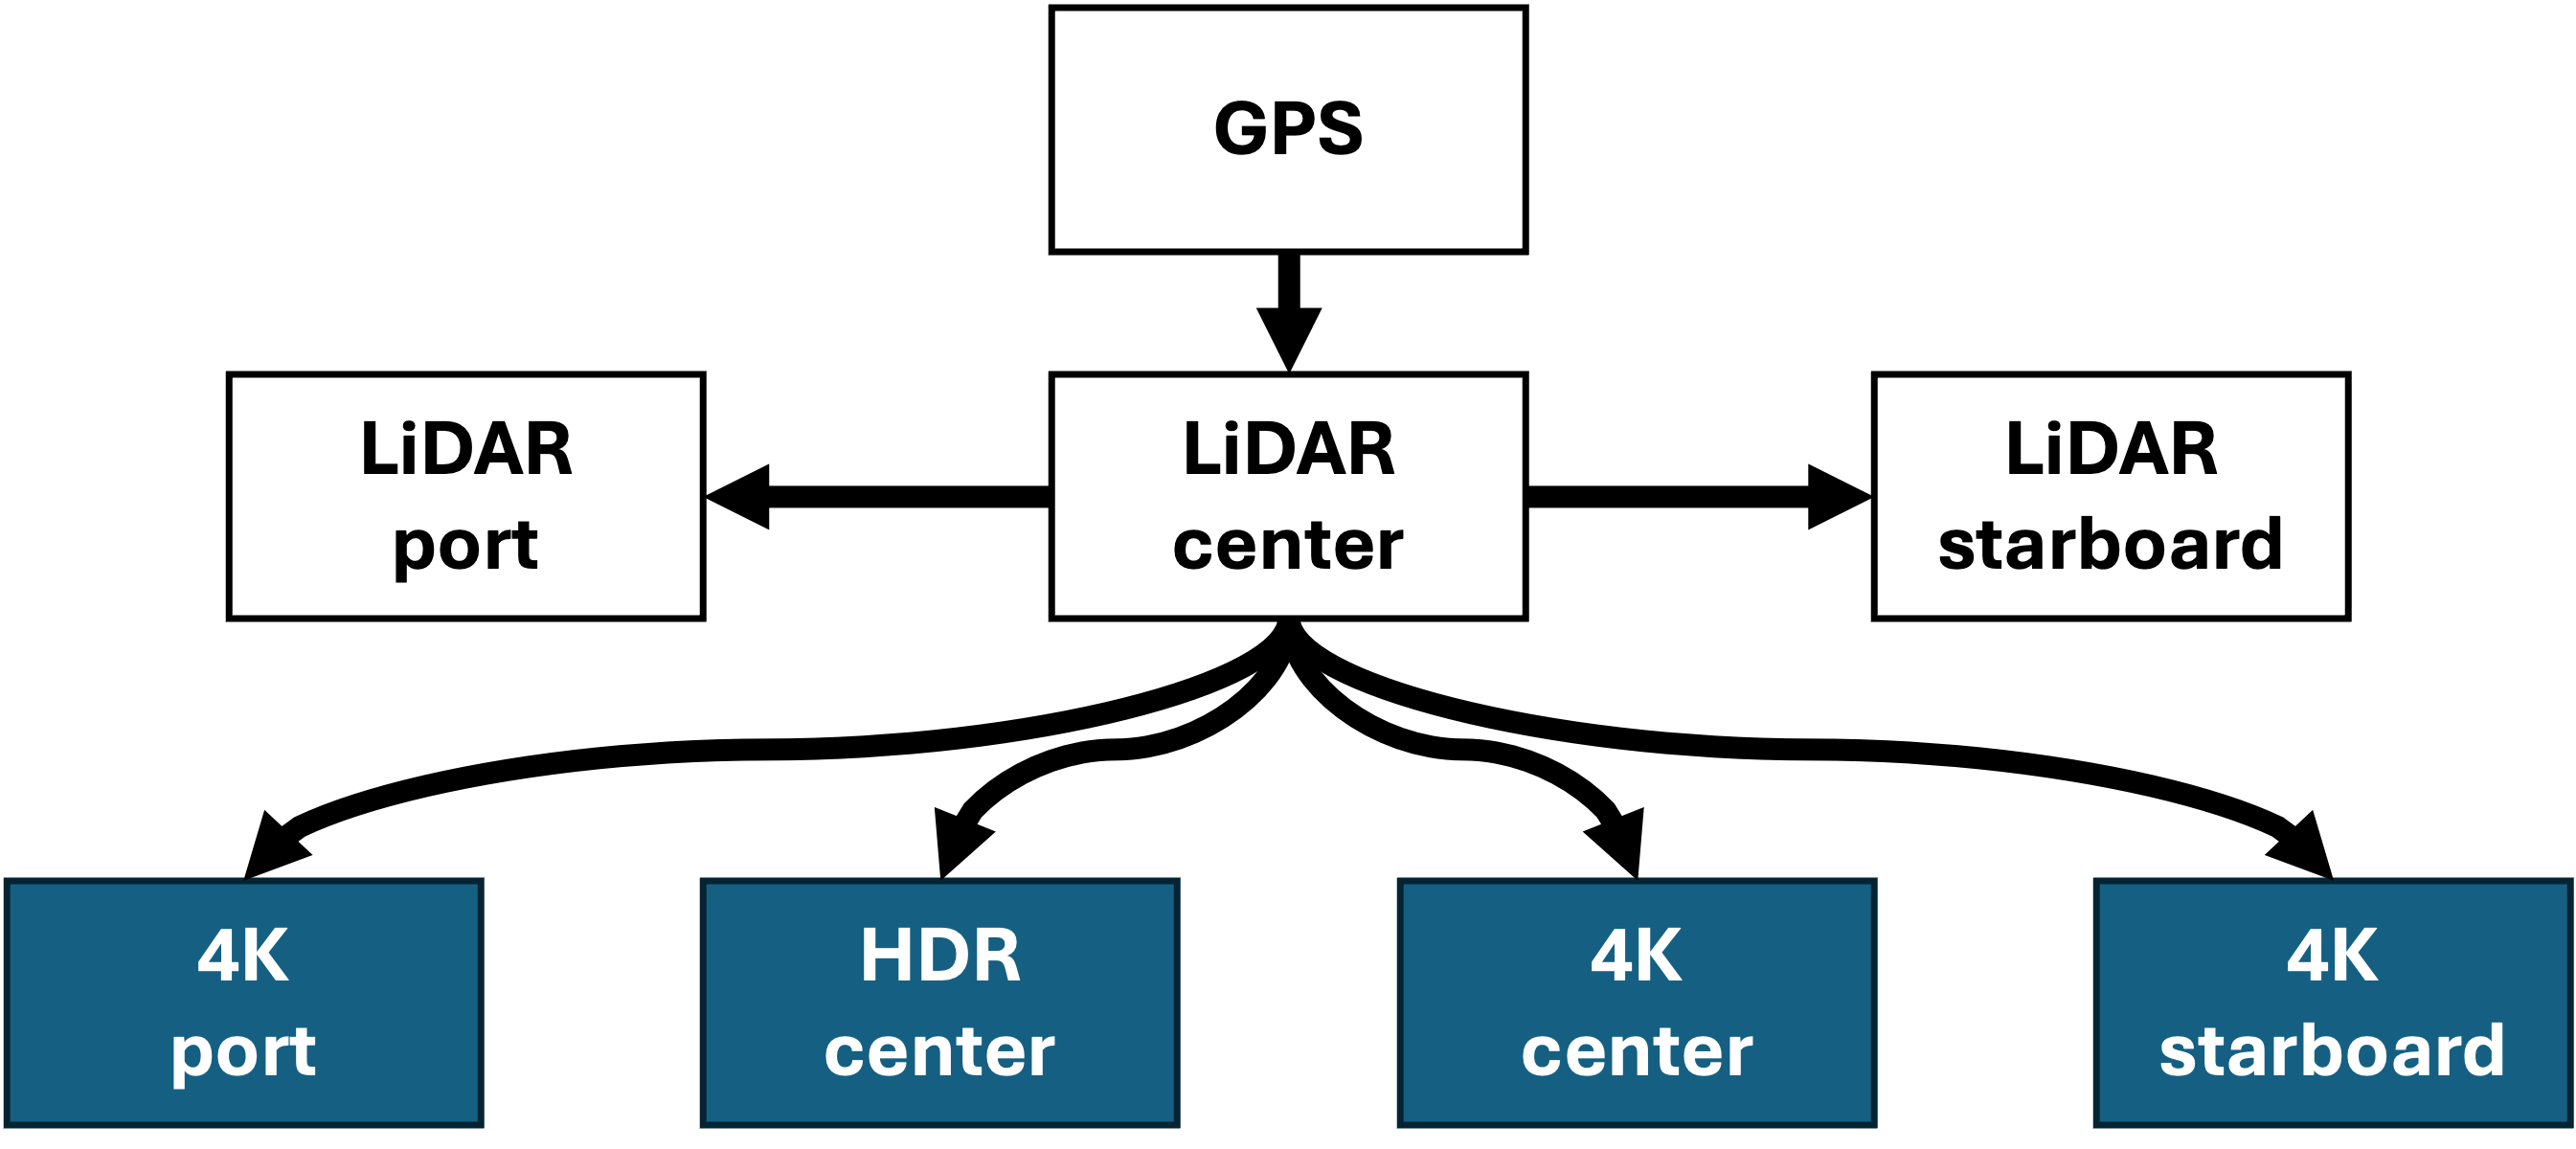
\includegraphics[width=0.75\textwidth]{Images/spatial_transforms.png}
\caption{A flowchart of transforms between sensor reference frames. Arrows indicate extrinsic transformations, and dark boxes indicate an additional intrinsic transform.}
\label{transform_diagm}
\end{figure}
%%%%%%%%%%%%%%%%%%%%%%%%%%%%%%

\section{Compute and LAN} \label{compute_lan}

The Minion platform's computing architecture consists of two primary systems: a main compute module housed in a waterproof Pelican case and a dedicated camera enclosure with integrated processing. The main compute module contains the Atlas PC and a 16-port network switch that aggregates all sensor and subsystem connections. The camera enclosure integrates a self-contained computing system responsible for camera data acquisition, video encoding, and timestamp synchronization with the vessel's global time reference. This modular architecture enables independent development and testing of the perception system while maintaining compatibility with the broader platform infrastructure.

\subsection{Camera Enclosure Computing Platform} \label{jetson_platform}

An NVIDIA Jetson AGX Xavier serves as the dedicated computer within the camera enclosure, handling all camera interface, video encoding, and network streaming operations. The Jetson was selected for its GPU acceleration capabilities, compact form factor, and native support for industrial camera interfaces including GMSL2 (Gigabit Multimedia Serial Link) required by the Leopard Imaging HDR camera.

The Jetson AGX Xavier features an 8-core ARM CPU, 512-core Volta GPU with 64 Tensor cores, and 32 GB of unified memory, providing sufficient computational resources for real-time video encoding of multiple simultaneous camera streams. The integrated GPU enables hardware-accelerated H.264/H.265 video encoding, reducing CPU load and network bandwidth requirements compared to uncompressed image transmission.

The Jetson connects directly to all cameras within the enclosure: the Leopard Imaging HDR camera via GMSL2 interface and three FLIR Blackfly S cameras via GigE Vision over Ethernet. Custom \ac{ROS} driver nodes execute on the Jetson to interface with each camera, configure acquisition parameters, capture frames, embed timestamps, encode video streams, and transmit encoded data to the vessel's main computer.

% A critical function of the Jetson platform is timestamp embedding for temporal synchronization. As described in Section~\ref{temporal_sync}, accurate sensor fusion requires camera frame timestamps to represent the actual moment of image capture referenced to a global time base. The Jetson system clock synchronizes to the vessel's \ac{GPS}-disciplined time reference via Network Time Protocol, then embeds synchronized timestamps into each video frame as supplemental encoded information (SEI) data within the H.264 stream. This approach ensures frame timestamps remain associated with image data throughout network transmission and decoding.

The camera enclosure design emphasizes modularity and research flexibility. The self-contained Jetson computer with local camera connections enables the perception system to be removed, modified, and tested independently of the Minion platform. Firmware updates, camera reconfiguration, and software development can proceed in the laboratory without requiring access to the full vessel. Network connectivity to the Minion platform occurs through a single Ethernet connection carrying both encoded video streams via \ac{RTP} and bidirectional \ac{NTP} for clock synchronization.

\subsection{Network Architecture} \label{network_structure}

% The Minion platform implements a hierarchical local area network (LAN) architecture connecting all computing resources and sensors. The network topology separates high-bandwidth sensor data streams from lower-rate command and control traffic while maintaining deterministic latency for time-critical communications.

The Atlas PC functions as the central computing node, hosting the primary \ac{ROS} environment, object detection algorithms, mission planning software, and data logging infrastructure. Atlas connects to the vessel LAN via a gigabit Ethernet switch that aggregates connections from all network-capable sensors and subsystems.

% Key network endpoints include:
% \begin{itemize}
% \item \textbf{Jetson AGX Xavier} (camera enclosure): Video streams and timestamp synchronization
% \item \textbf{Livox Horizon \ac{LiDAR} units} (3 sensors): UDP point cloud data at 100 Hz per sensor
% \item \textbf{PinPoint \ac{GPS}/\ac{IMU}}: Pose data and Network Time Protocol time reference
% \item \textbf{Velodyne HDL-32E \ac{LiDAR} units} (3 sensors): UDP point cloud data for navigation
% \item \textbf{Shore connection}: Ground station monitoring and remote access during development
% \end{itemize}

Static IP address assignment ensures deterministic routing and simplifies network administration. The PinPoint \ac{GPS}/\ac{IMU} is configured with IP address 201.7.90.30 and designated as the authoritative Network Time Protocol server for the vessel. All other computing resources synchronize to this \ac{GPS}-disciplined time source to establish a common temporal reference.

This \ac{RTP}-based approach was developed to address network latency issues observed with alternative solutions. Open-source plugins such as GStreamer-based GSCam and NVIDIA's DeepStream SDK were evaluated but found insufficient for Minion's specific requirements. The custom implementation provides granular control over video encoding parameters (resolution, frame rate, bitrate, compression method) and ensures embedded timestamps survive the encoding-transmission-decoding pipeline without modification.

Point cloud data from the three Livox Horizon \ac{LiDAR} sensors arrives as \ac{UDP} packets transmitted directly to the Minion LAN at 100 Hz per sensor. The Livox SDK executing on Atlas receives these streams, parses binary point cloud messages, and publishes data to \ac{ROS} topics for consumption by perception algorithms. 

\begin{figure}[htbp]
    \centering
    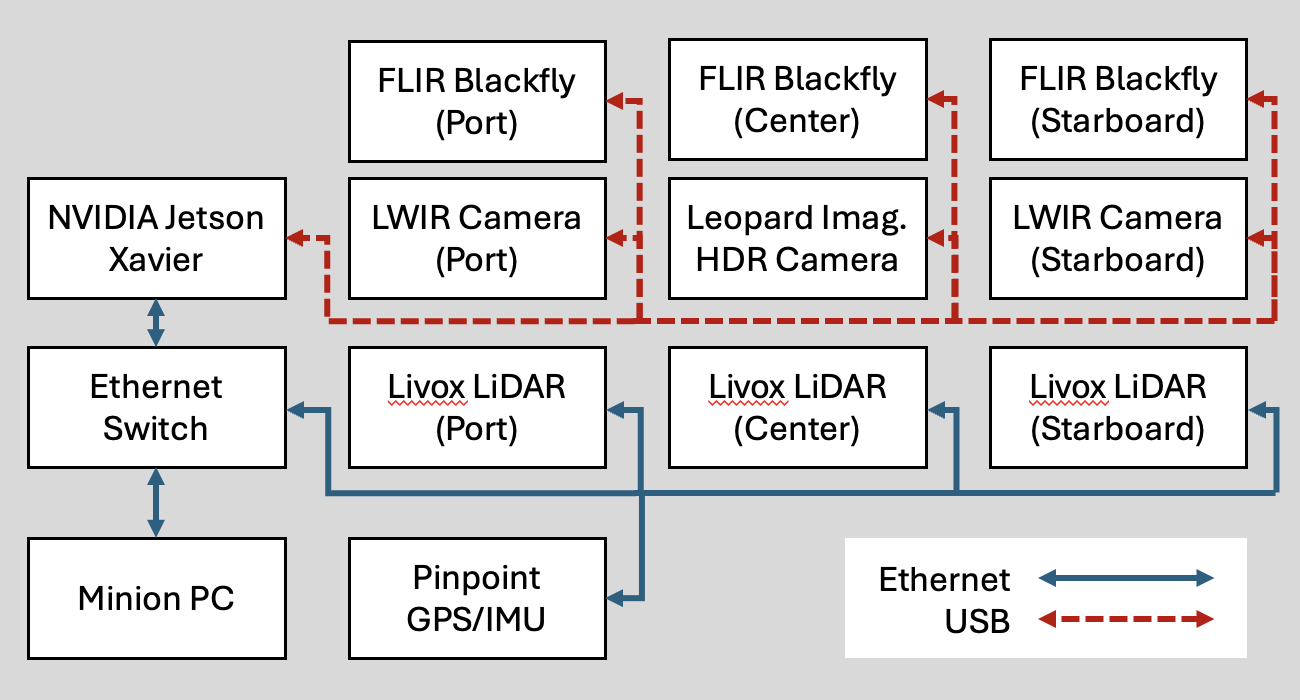
\includegraphics[width=0.85\textwidth]{Images/network_diagram.png}
    \caption{Block diagram of the network architecture of the \ac{USV}. Red dashed arrows indicate USB connections and blue solid arrows indicate Ethernet-connected blocks.}
    \label{fig:network_diag}
\end{figure}

Bandwidth analysis for the forward perception system indicates peak data rates of approximately:

\begin{table}[htbp]
\centering
\caption{Peak data rates for forward perception sensors}
\label{tab:network_bandwidth}
\begin{tabular}{lccc}
\hline
\textbf{Sensor} & \textbf{Specifications} & \textbf{Quantity} & \textbf{Data Rate} \\
\hline
Livox \ac{LiDAR} & 480k pts/sec, dual return, 100 Hz, 16 bytes/pt & 3 & $\approx$ 23 Mbps \\
HDR Camera & H.264, 5 fps, 2880$\times$1860 & 1 & 8--12 Mbps \\
% FLIR Cameras & H.264, 31 fps, 4000$\times$3000 & 3 & 15--25 Mbps each \\
\hline
\end{tabular}
\end{table}

Total sustained network load during perception operations remains well below the gigabit Ethernet capacity, ensuring minimal packet loss and deterministic latency.

Quality of Service (QoS) configuration prioritizes time-sensitive traffic such as \ac{GPS}/\ac{IMU} pose updates and Network Time Protocol synchronization packets over bulk data transfers. This ensures clock synchronization accuracy is maintained even during periods of high sensor data throughput.

The hierarchical network architecture with segregated sensor and control traffic, static addressing for deterministic routing, and low-latency \ac{UDP}-based protocols establishes a robust foundation for real-time multi-modal perception and autonomous operation.

\section{Data Collection}

Integrating the spatial precision of LiDAR data and the dense pattern information and color discernment of camera data can facilitate a much more accurate interpretation of the system environment. However, to fuse data from both modalities, these sensors must be calibrated through geometric transforms and have their measurement timing synchronized. This ensures that anything in view of either sensor can be easily cross-referenced by the other for additional information.
    
\subsection{Calibration}

First, this process entailed precise intrinsic and extrinsic calibrations to reduce the geometric error between the LiDAR and camera reference frames. 
Second, custom software was written to stream the video data to overcome network latency issues and achieve the levels of temporal accuracy required. 
This software encodes the system time that each frame is captured into the video data, which is then streamed using the \ac{RTP} from the camera enclosure to Minion's main CPU. 
On Minion, the video stream is decoded, and the image frame and embedded timestamp are published as a Robotic Operating System (ROS) message. 
These enhancements enable the accurate fusion of information between camera and LiDAR sensors at a frame rate of 5 fps.

Before the data from the camera and LiDAR sensors can be combined, each device needs to be spatially calibrated through extrinsic and intrinsic transforms. 
This ensures that the scale and position of objects seen by either sensor type can be placed into a common reference frame. 
Additionally, the data received from each device should agree upon what moment in time the data represents. 
Prior to this year's competition, latency in the video signal was compensated for by adjusting its timestamp with a constant offset, and while this method was sufficient when the USV was stationary, it created significant errors during rapid motion, especially turning.

\subsubsection{Camera Intrinsics}

Camera intrinsics refer to a camera's unique properties which define the path of light through its optical path.
These properties can functionally define the path of any ray of light through the camera lens to the exact location on the camera sensor and provide a geometric translation from a position in the 3-dimensional camera frame to a 2-dimensional pixel location in the image frame. 
It is generally represented as a $3 \times 3$ matrix as:
$$
\begin{bmatrix}
    f_x & s & c_x \\
    0 & f_y & c_y \\
    0 & 0 & 1
\end{bmatrix}
$$
where $(f_x, f_y)$ is the focal length of the camera lens in pixels, $(c_x, c_y)$ is the $(x,y)$ position (measured in pixels) in the image frame that is centered in the optical path, known as the principal point, and skew $s$ is the angle between the vertical and horizontal axis of the image frame that is generally assumed to be $s = 0$. 
Radial distortion is the spherical abortion caused by the camera lens and is represented as either one, two, or three constants of a polynomial $k_1,k_2,k_3$, where:
\begin{align*}
x_{distorted} & = x(1+k_1r^2+k_2r^4+k_3r^6)\\
y_{distorted} & = y(1+k_1r^2+k_2r^4+k_3r^6)\\
r^2 & = x^2+y^2
\end{align*}

While these values are generally published as part of the camera specifications, calibration is still required to account for manufacturing tolerances. A common method to perform this calibration is through homography, and involves capturing several images of a checkerboard pattern in multiple positions within the image frame \textcolor{blue}{The MathWorks, Inc. (2024). MATLAB version: 24.1.0 (R2024b)}.

MATLAB's Camera Calibration application uses an algorithm based on this technique, which identifies intersecting points made by the checkerboard squares and the measured distance in pixels. 
This information is cross-referenced with the physical dimensions of the checkerboard.
This tool estimates the camera's intrinsic properties by minimizing the error between the observed checkerboard patterns and projected points through a pin-hole camera model \textcolor{blue}{The MathWorks, Inc. (2024). Computer Vision Toolbox version: 24.1 (R2024a)}.
However, the accuracy of this method is dependent on the quality of the calibration data used. 
Minion's calibration dataset consisted of 23 instances of simultaneous LiDARscans and camera recordings with the checkerboard placed at various locations and distances within each camera's view. 
While only only data from the camera sensors are required to calibrate intrinsics, the LiDAR data is captured simultaneously for extrinsic calibration.
A composite of several images taken during Minion's camera calibration is provided in figure \ref{fig:camera_calib}.

\begin{figure}[htbp]
\centering
\begin{subfigure}[t]{0.45\textwidth}
    \centering
    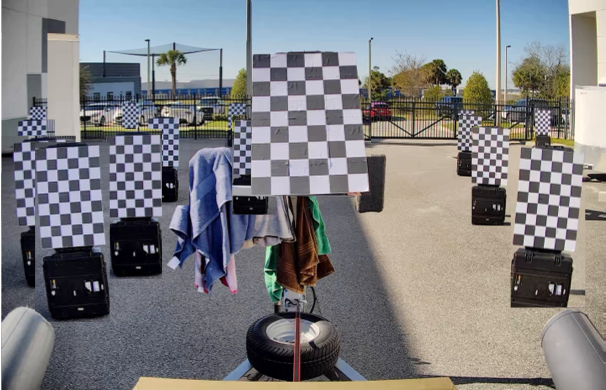
\includegraphics[width=\textwidth]{Images/checkerboard.png}
    \caption{Composite image of checkerboard locations during calibration as seen by the HDR camera}
    \label{fig:chkrbds_vision}
\end{subfigure}
\hfill
\begin{subfigure}[t]{0.45\textwidth}
    \centering
    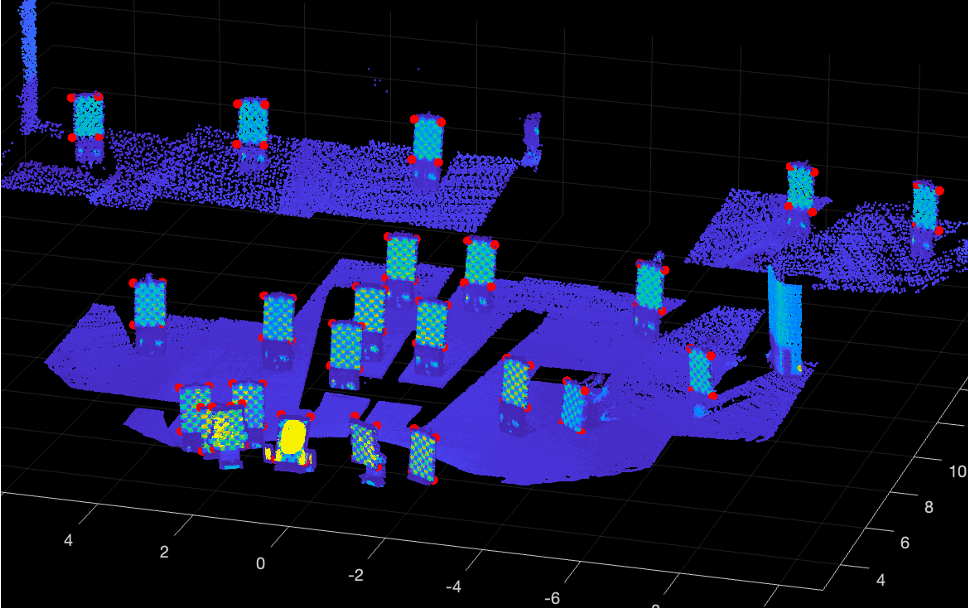
\includegraphics[width=\textwidth]{Images/lidar_calib.png}
    \caption{Composite image of the same checkerboard locations as seen by LiDAR}
    \label{fig:chkrbds_lidar}
\end{subfigure}
\caption{Comparative visualization of checkerboard co-location as seen by visual and LiDAR modality}
\label{fig:camera_calib}
\end{figure}

\begin{figure}[htbp]
    \centering
    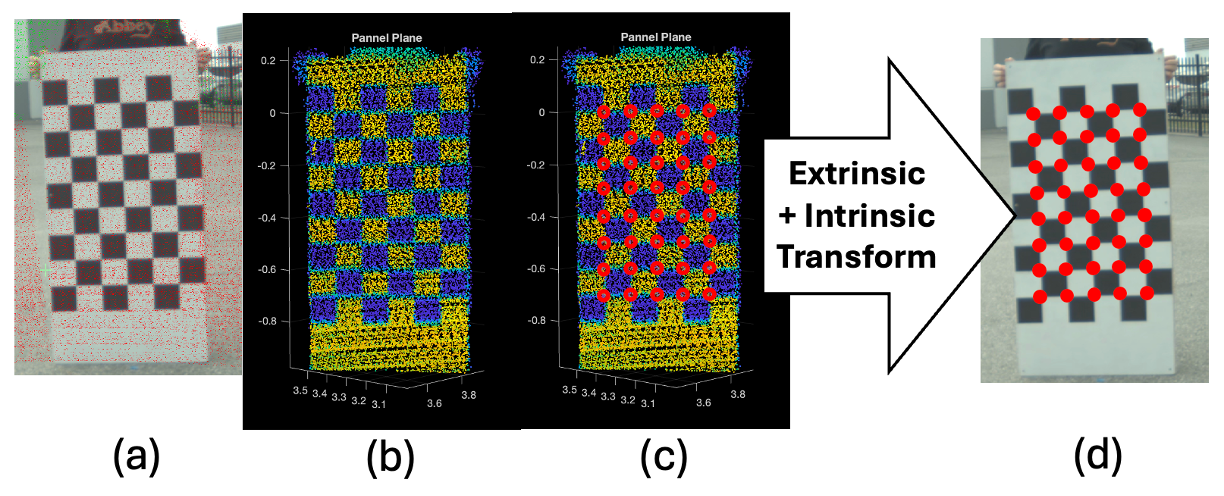
\includegraphics[width=0.9\textwidth]{Images/transform.png}
    \caption{caption}
    \label{fig:lidar_cam_calibration}
\end{figure}

            
\subsubsection{Camera Extrinsics}

For camera-to-LiDAR calibration, the checkerboard calibration dataset is reused from the camera intrinsic calibration.
One second of LiDAR scan data is isolated for each position of the checkerboard pattern to obtain a more dense point cloud and then loaded into the LiDAR Calibration tool within MATLAB.
% Data from sensor pairs (e.g. the port viewing LiDAR is paired with the port viewing 4k camera, and the center LiDAR is paired with center 4k and center HDR cameras) are loaded into MATLAB using the LiDAR Calibration application.
This function co-locates the three-dimensional checkerboard pattern from the image frame using the identified camera intrinsics and the point cloud data and then estimates the transform between them. 
This function identifies the inner corners of the checkerboard, co-locates this information in the camera and LiDAR frames, and estimates the transform between them \textcolor{blue}{The MathWorks, Inc. (2024). Computer Vision Toolbox version: 24.1 (R2024a)}. 
This initial calibration is shown in Figure \ref{fig:lidar_cam_calibration} by projecting the inner checkerboard corners detected in the images (red) into the LiDAR point cloud data.
While imperfect, this process provides a good first estimate of the extrinsic transformation between the HDR camera frame and LiDAR sensor frame.

\begin{figure}[htbp]
    \centering
    \begin{subfigure}{0.85\textwidth}
        \centering
        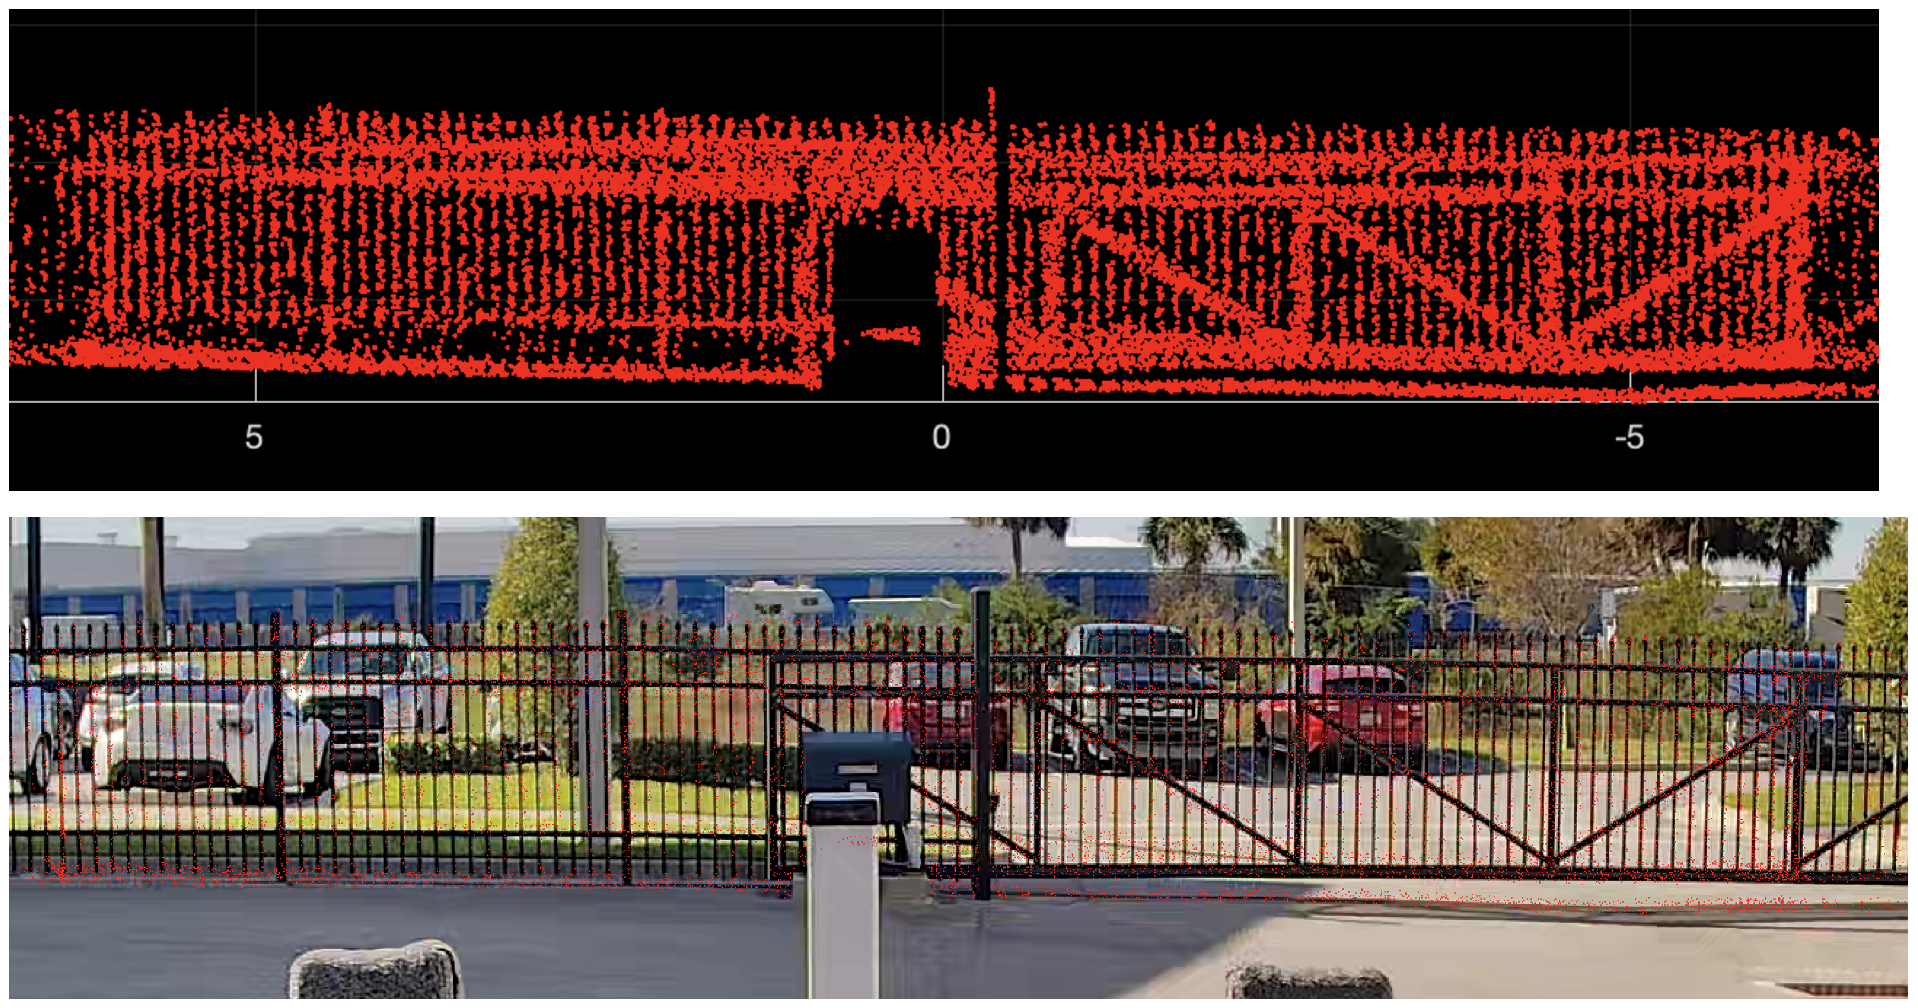
\includegraphics[width=\textwidth]{Images/LiDAR_calib_fence.png}
        \caption{Isolated LiDAR points of fencing (top) projected as red pixels onto the image frame (bottom).}
        \label{fig:LiDAR_calib_fence}
    \end{subfigure}
    
    \vspace{0.5em} % small vertical space between images

    \begin{subfigure}{0.85\textwidth}
        \centering
        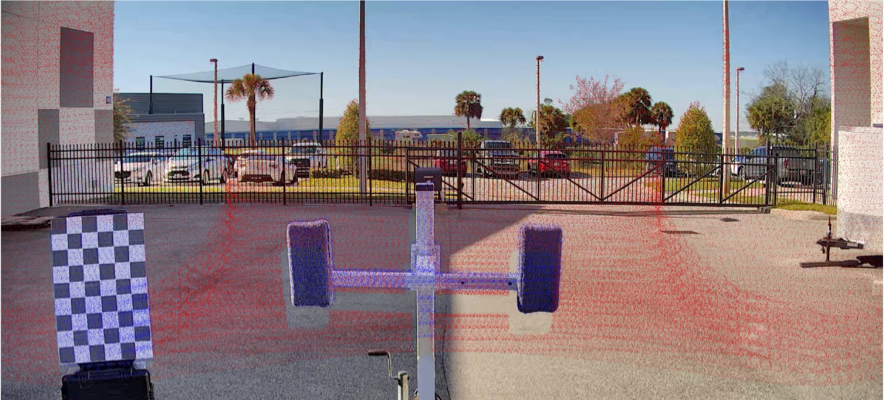
\includegraphics[width=\textwidth]{Images/LiDAR_calib_composite.png}
        \caption{LiDAR points projected onto the image frame as red pixels, with isolated foreground object points in blue}
        \label{fig:LiDAR_calib_composite}
    \end{subfigure}

    \caption{Manual refinement of Camera to LiDAR frame extrinsic transform evaluated by aligning isolated object points within the image frame.}
    \label{fig:LiDAR_calib_combined}
\end{figure}

These initial values are refined through a manual process by projecting LiDAR data onto the image frame and inspecting how the LiDAR points align with objects within the \ac{FOV} such as walls, trees, fencing, and lamp posts, as shown in Figures~\ref{fig:LiDAR_calib_fence} and~\ref{fig:LiDAR_calib_composite}.
The final extrinsic transform is provided in Table~\ref{tbl:extrinsic}.

            
\subsubsection{Livox Extrinsics} \label{lidar_extrinsic}
To identify object positions in a different reference frame than it is measured requires an extrinsic transform between the frames. 
This transform defines the translation and rotation (yaw, pitch, roll, $x,y,z$) to make one frame match another and is represented by quaternions or Euler angles.
For Minion, an extrinsic transform is used between the port and starboard facing Livox devices to the central forward facing Livox to create a unified point cloud. Each camera also receives an extrinsic transform to the Livox reference frame.
A flowchart of these transforms is provided in Figure \ref{transform_diagm}.
% required between the center Livox frame and each of the four camera sensors as well as the port and starboard Livox devices.
% Each sensor is calibrated to an $x$-up, $z$-forward, $z$-down reference frame located at the origin of the forward-facing center Livox Horizon, see \ref{transform_diagm}. 

% Each Livox Horizon is equipped with a inertial measurement unit (IMU) to ensure that the final reference frame is level.

% A similar 
% A series of LiDAR scans are simultaneously captured with video from each camera.
% Objects are accurately located within the data sets of both sensor types to perform the spatial calibration between them.

LiDAR-to-LiDAR calibration is performed with first-party software Livox Viewer, available through the manufacturer's website.
This software provides a real-time view of the LiDAR returns and adjustment of the extrinsic calibration for each sensor.
The large flat surfaces of the laboratory, as well as the larger paved area behind the laboratory, both provide excellent large and flat surfaces that allow them to be easily co-located by manually adjusting the extrinsic values.
As shown in Figure~\ref{transform_diagm}, the port and starboard Livox Horizons are transformed into the \textcolor{blue}{center livox} frame, and the extrinsic transforms required to do so are stored in the non-volatile memory of each sensor. This means that once calibrated, the raw point cloud data from each sensor is transmitted in the \textcolor{blue}{center livox} frame.




\begin{table}[ht]
\caption{Final Transforms to Center Livox frame}
\label{extrinsics}
\centering
\begin{tabular}{l|cccccc}
% \hline
Sensor &  roll & pitch & yaw & $x$ & $y$ & $z$\\
\hline \hline 
Livox (port)  & -4.14 & 1.47 & 42.97 & -0.057 & 0.169 & 0\\ \hline
% Livox (fwd) & 0 & 1.63 & 0 & 0 & 0 & 0\\ \hline
Livox (stbd) & 4.25 & 1.85 & -42.6 & -0.057 & -0.169 & 0\\ \hline
\hline

% 4K (port) &  -88.35 &   0.84 & -97.16 & -0.031 & 0.155 & 0.159\\ \hline
HDR (fwd) & 103.85 & -0.69 & 88.83 & -0.032 &0.115 & 0.098\\ \hline
% 4K (fwd) & -88.31&    0.98&  -97.33& -0.023 & 0.095& 0.19\\ \hline
% 4K (stbd) & -88.35&    0.84&  -97.16 & -0.32 & 0.15& 0.16\\ \hline
\end{tabular} \label{tbl:extrinsic}
\end{table}
            
        \subsection{Synchronization} \label{sync}
        
            \subsubsection{Clock Synchronization} \label{clock_sync}

Accurate temporal alignment of observations from multiple sensors operating with independent clocks requires that all sensors share a common time reference. The Minion autonomous surface vessel implements a hierarchical clock synchronization architecture that distributes GPS-disciplined time from a single authoritative source through a cascade of increasingly precise synchronization protocols. This multi-tier approach balances the accuracy requirements of different sensor types---millisecond-level precision for camera frames versus microsecond-level precision for LiDAR points---while maintaining architectural simplicity and operational reliability.
% The time distribution system employs a three-tier hierarchy: GPS Time →\rightarrow
% → \ac{NTP} Distribution →\rightarrow
% → \ac{PTP} Distribution. 
The Pinpoint GPS/INS receiver extracts time from GNSS satellite signals, providing UTC time with typical accuracy of 10--100 nanoseconds. Operating at IP address 201.7.90.30 on the vessel LAN, the GPS unit functions as a stratum-1 \ac{NTP} server, indicating direct attachment to a reference clock. One Atlas PC (Minion A or Minion B) synchronizes its system clock to the Pinpoint GPS via Network Time Protocol using the Chrony daemon, then operates as an \ac{NTP} server for other platform computing resources. The Atlas PC maintains synchronization accuracy typically within 1--10 milliseconds of GPS time, limited primarily by network latency rather than GPS accuracy. The NVIDIA Jetson Xavier camera enclosure computer synchronizes to the Atlas \ac{NTP} server, inheriting GPS-disciplined time for video frame timestamping.

The cascaded architecture ensures that all sensors reference the same GPS time source despite employing different synchronization protocols optimized for their respective accuracy requirements.
\ac{NTP} provides adequate accuracy ($1-10$ ms) for video frame timestamps given the $10$ Hz sampling rate, while LiDAR sensors demand substantially higher timing precision. 
Each Livox Horizon unit incorporates IEEE 1588 \ac{PTP} support for sub-microsecond clock synchronization, with the Jetson Xavier functioning as the \ac{PTP} grandmaster. 
The Linux \ac{PTP} project's \texttt{ptp4l} daemon executes on the Jetson Xavier, broadcasting \ac{PTP} timing packets over the camera enclosure Ethernet network segment that includes the three Livox sensors. 
\ac{PTP} achieves microsecond-level accuracy (typically $1-10 \mu s$) through hardware-timestamped network packets and symmetric delay compensation, meeting the stringent timing requirements for spatial measurement sensors. 
Both the Jetson Xavier and Livox Horizon sensors employ network interfaces with hardware timestamp support, enabling the symmetric delay measurement required for accurate \ac{PTP} synchronization.

To prevent recording with uncalibrated timestamps, the video encoding pipeline implements mandatory synchronization verification before launching camera capture processes. The startup script executes two checks with defined timeouts: first, a 60-second verification that Chrony synchronization is established with ``Normal'' leap status and active connection to the upstream \ac{NTP} source; second, a 30-second confirmation that the system clock reflects actual calendar time rather than a default epoch value. Only after both checks pass does the startup script launch the GStreamer video encoding pipelines, preventing the collection of video data with incorrect temporal references that would compromise subsequent sensor fusion analysis.
            
\subsubsection{Video Pipeline} \label{video pipeline}
            
The video processing pipeline implements a sophisticated timestamp embedding methodology that preserves GPS-synchronized timing information through the entire encoding, transmission, decoding, and recording chain. This approach embeds absolute system timestamps directly into the H.264/H.265 video bitstream as Supplemental Enhancement Information \ac{SEI} metadata, ensuring that timing information remains inseparably bound to the corresponding video frames throughout all processing stages.
Standard video processing workflows typically assign timestamps relative to stream start time, which proves inadequate for multi-sensor fusion applications requiring absolute temporal references. The GStreamer multimedia framework, employed for video capture and encoding, operates with timestamps measured from the beginning of each stream---a convention suitable for multimedia playback synchronization but incompatible with the requirement to associate video frames with LiDAR observations timestamped in GPS time. Several approaches for associating absolute timestamps with video frames were evaluated, including external CSV logging, \ac{RTP} timestamp modification, and visible video overlays. The in-band metadata approach via \ac{SEI} \ac{NAL} units was selected based on critical advantages: timestamps persist through network network transmission; each frame carries its own embedded timestamp with no possibility of misalignment; \ac{SEI} messages comply with H.264/H.265 specifications, making them invariant to video encoding software versions, as well as not requiring custom metadata.
The video encoding pipeline executes on the NVIDIA Jetson Xavier, exploiting hardware-accelerated video encoding engines to achieve real-time compression of the HDR video stream. The GStreamer pipeline structure for each camera follows the sequence listed in~\ref{vide_encode}: 

\begin{algorithm}
\caption{Transmit Pipeline (Jetson Xavier)}
\begin{algorithmic}[1]
\State \texttt{v4l2src (camera capture)}
\State $\rightarrow$ \texttt{capsfilter (video/x-raw, 2880x1860, 25 fps)}
\State $\rightarrow$ \texttt{[timestamp capture probe: sample GPS-sync system time]}
\State $\rightarrow$ \texttt{videoconvert (color space conversion)}
\State $\rightarrow$ \texttt{videorate (downsample to 5 fps)}
\State $\rightarrow$ \texttt{capsfilter (video/x-raw, 2880x1860, 5 fps)}
\State $\rightarrow$ \texttt{x264enc / x265enc (hardware-accelerated compression)}
\State $\rightarrow$ \texttt{[SEI insertion probe: embed timestamp as NAL unit]}
\State $\rightarrow$ \texttt{rtph264pay / rtph265pay (RTP packetization)}
\State $\rightarrow$ \texttt{RTSP server (network transmission)}
\end{algorithmic} \label{vide_encode}
\end{algorithm}

\begin{algorithm}
\caption{Receive Pipeline (Atlas PC)}
\begin{algorithmic}[1]
\State \texttt{udpsrc (UDP network reception, port 5603)}
\State $\rightarrow$ \texttt{rtph264depay / rtph265depay (RTP depacketization)}
\State $\rightarrow$ \texttt{h264parse / h265parse (bitstream parsing)}
\State $\rightarrow$ \texttt{[SEI extraction probe: recover embedded timestamp]}
\State $\rightarrow$ \texttt{avdec\_h264 / avdec\_h265 (software decoding)}
\State $\rightarrow$ \texttt{videoconvert (format conversion)}
\State $\rightarrow$ \texttt{videoscale (optional resolution scaling)}
\State $\rightarrow$ \texttt{appsink (application callback)}
\State $\rightarrow$ \texttt{ROS sensor\_msg/Image publication}
\end{algorithmic} \label{video_decode}
\end{algorithm}

This architecture captures the timestamp as close to image frame capture as possible, and holds the information until after the video is down-sampled and encoded.
A custom GStreamer metadata system propagates absolute timestamps through the processing pipeline. A pad probe attached to the source pad of \texttt{v4l2src} captures system time for each incoming video buffer using \texttt{gettimeofday()}, sampling the \ac{NTP}-synchronized system clock to obtain GPS-disciplined time. The resulting timestamp is attached to the GStreamer buffer as custom metadata that persists through subsequent pipeline elements. When the \texttt{videorate} element reduces the 25 fps input to 5 fps output, the metadata transform callback ensures that the timestamp from the selected buffer is copied to the output frame, preserving the original capture time even when frames are dropped.
The H.264 video compression standard defines \ac{SEI} as a mechanism for carrying metadata alongside compressed video. 
The timestamp \ac{SEI} message employs the unregistered user data payload type (type 5), consisting of the timestamp (8 bytes) encoded as a \texttt{uint64\_t} value representing milliseconds since Unix epoch, followed by 8 bytes of padding to complete a 16-byte payload. 
A pad probe attached to the source pad of the H.264 video encoder (\texttt{nvv4l2h264enc}) constructs and inserts \ac{SEI} \ac{NAL} units before each encoded frame.  
The \ac{SEI} \ac{NAL} unit is prepended to the encoded frame buffer, maintaining the association between timestamp and image content through all subsequent processing stages including \ac{RTP} packetization and \ac{UDP} transmission.

Video transmission from the Jetson to Atlas employs \ac{RTSP} over \ac{UDP} to minimize latency and avoid transmission delays associated with TCP acknowledgment mechanisms. The Atlas PC receives and decodes the \ac{RTSP} streams through a complementary GStreamer pipeline into ROS image messages. A pad probe attached to the H.264/H.265 parser element extracts embedded timestamps from \ac{SEI} \ac{NAL} units before decoding. Due to potential fragmentation of \ac{NAL} units across GStreamer buffers, the extraction implementation accumulates incoming data until complete \ac{NAL} units can be identified and parsed. The extraction logic identifies \ac{SEI} \ac{NAL} units by type, verifies the custom UUID, and extracts the 8-byte timestamp value.

The \texttt{appsink} element at the end of the receive pipeline provides decoded video frames to the application. A callback function executes for each frame, extracting the frame data and publishing it as a ROS \texttt{sensor\_msg/Image} message with the previously extracted \ac{SEI} timestamp converted from millisecond Unix epoch time to ROS time format. 
% The ROS \texttt{image\_transport} package provides efficient image message publication with automatic transport plugin support, creating raw and compressed image topics. 
% Critically, the \ac{SEI}-derived timestamp is applied to all transport variants, ensuring temporal accuracy regardless of which compressed format is recorded.
The video pipeline achieves real-time performance encoding three simultaneous 2880$\times$1860 pixel camera streams at 10 fps with measured end-to-end latency averaging 127 milliseconds from frame capture to ROS publication. Hardware encoding latency ranges from 10--30 ms per frame for H.264/H.265, with network transmission latency of 1--5 ms over the Gigabit LAN and negligible \ac{SEI} insertion overhead (<1 ms). Zero frame drops and zero frame repetition under normal operation confirm the temporal stability of the implementation. The timestamps embedded via \ac{SEI} reflect the GPS-synchronized system clock on the Jetson Xavier at the moment of frame capture, with accuracy depending on the \ac{NTP} synchronization quality between Jetson and Atlas PC, typically achieving 1--10 millisecond accuracy relative to GPS time.
            
            \subsubsection{Temporal Drift} \label{temporal_drift}
            
    \section{Data Output}


\section{Compute Hardware and Network} \label{sec:Atlas_LAN}

The Minion autonomous surface vessel employs a distributed computing architecture that balances real-time processing requirements with operational flexibility and redundancy. 
The computing infrastructure consists of high-performance workstation computers serving as the primary processing platforms, an embedded computer integrated with the camera sensors for video encoding and streaming, and a \ac{GbE} \ac{LAN} connecting all systems and sensors. 
% This architecture distributes computational workloads according to sensor proximity and processing requirements while maintaining centralized coordination through the Robot Operating System middleware. 
The following subsections detail the hardware specifications, system architecture, and network infrastructure that enable real-time multi-modal perception for maritime object detection and sensor fusion.

%%%%%%%%%%%%%%%%%%%%%%%%%%%%%%%%%%%%%%%%%%%%%%%%%%%%%%%%%%%%%%%%%%%%
\subsection{Atlas} \label{atlas}

The primary computing infrastructure consists of two identical high-performance workstation computers designated Minion A and Minion B.
These systems, built on enterprise-grade PC hardware, provide the computational resources necessary for real-time sensor data processing, object detection algorithm execution, and autonomous navigation decision-making.
The dual-computer configuration provides operational redundancy, allowing hot-swapping between systems for software development, testing, and failover scenarios without requiring vessel downtime.

\subsubsection{CPU and Memory}
Each Atlas PC, designated Minion-A and Minion-B, features computing hardware selected to meet the demanding real-time requirements of multimodal perception and autonomy.
Table \ref{table:Minion_hardware} presents the key hardware specifications for the Atlas.% computing platform.

The six-core Xeon processor with Hyper-Threading provides twelve logical threads, offering sufficient parallel processing capability to handle simultaneous operation of LiDAR point cloud processing, computer vision algorithms, sensor fusion, and navigational planning.
Operating at 3.50 GHz base frequency with 15 MB of shared L3 cache, the processor provides substantial single-threaded performance for latency-sensitive perception tasks while enabling multi-threaded parallelism for batch processing operations.
The processor's support for AVX2 vector instructions accelerates numerical computation common in point cloud transformation and sensor fusion algorithms.

The 16 GB ECC memory capacity, configured in quad-channel DDR4-2133 with four 4 GB modules, provides sufficient capacity to store a large cache of LiDAR and video image data in the form of \ac{ROS} messages (see Section \ref{sensor_data}), enabling rapid access and parsing of large point clouds.% as discussed in Chapter \ref{realtime_object_detection}.
Error-correcting code memory improves system reliability for long-duration autonomous operations where memory corruption could compromise navigation safety or data integrity.
The quad-channel memory configuration provides 68 GB/s aggregate memory bandwidth, reducing bottlenecks when multiple perception algorithms access shared sensor data simultaneously.

\subsubsection{GPU}
The NVIDIA GTX 1080 GPU features 2560 CUDA cores based on the Pascal architecture and 8 GB of GDDR5X memory, accelerating both machine learning inference for object detection and point cloud processing operations.
The Pascal architecture provides CUDA compute capability 6.1, enabling efficient execution of YOLOv8 convolutional neural networks and GPU-accelerated image preprocessing described in Chapter \ref{realtime_object_detection}.
Hardware video decode engines offload H.264 video decompression from the CPU, enabling the Atlas PC to receive and process multiple camera streams simultaneously while maintaining CPU resources for perception algorithms.

\subsubsection{Storage}
High-speed solid-state storage provides the throughput necessary to record multiple synchronized sensor streams to disk during data collection operations.
Recording sessions simultaneously capture raw LiDAR point clouds, compressed video streams from three cameras, GPS/INS pose messages, and timestamped detection results, generating aggregate data rates that can exceed hundreds of megabytes per second.
% The storage subsystem must sustain these write rates for extended periods without buffer overflow or frame dropping.

\subsubsection{Network Connectivity}
The Atlas platform features extensive network connectivity with six \ac{GbE} ports, enabling flexible network architecture design. %plus 802.11ac WiFi
A PCIe expansion card provides four additional \ac{GbE} interfaces %. with hardware support for IEEE 1588 Precision Time Protocol timestamping, 
enabling future expansion of sensor networks or integration of additional computing nodes.
The Intel I210 network controller serves as the primary vessel LAN interface, connecting the Minion PC to the rest of the network, and the Intel I218-LM network card provides additional connectivity for external networks or redundant communication paths.

% at static IP address 201.7.90.17 to the Pinpoint GPS/INS at 201.7.90.30, the Jetson Xavier camera enclosure at 201.7.90.147, and the three Livox LiDAR sensors configured via DHCP.
% The Broadcom BCM4360 802.11ac WiFi adapter enables remote access and diagnostics during dock-side operations, though WiFi is not used for real-time sensor data transmission due to latency and reliability constraints.

\begin{table}[htpb]
\centering
\caption{Minion A/B PC Hardware Specifications}
\begin{tabular}{ll}
\hline
\multicolumn{2}{c}{Minion PC - Hardware Specification} \\
\hline
\hline
Processor (CPU) & Intel Xeon E5-1650 v3 \\
CPU Cores & 6-core / 12-thread, 3.50 GHz \\
% CPU Architecture & Haswell-EP, 15 MB L3 Cache \\
Graphics (GPU) & NVIDIA GeForce GTX 1080 \\
GPU Memory & 8 GB GDDR5X, 2560 CUDA cores \\
Memory (RAM) & 16 GB DDR4 (quad-channel) \\
Storage (Primary) & 256 GB NVMe SSD \\
Network Interface & (6x) Gigabit Ethernet \\% + 802.11ac WiFi \\
% Primary Vessel LAN & Intel I210 GbE (201.7.90.17) \\
% \hline
% \multicolumn{2}{c}{Minion-A Operating System} \\
% \hline
% Primary OS & Ubuntu 22.04 LTS \\
% ROS Version & ROS 2 Humble\\
% \hline
% \multicolumn{2}{c}{Minion-B Operating System} \\
% \hline
% Primary OS & Ubuntu 20.04 LTS \\
% ROS Version & ROS 1 Noetic \\
\hline
\end{tabular}
\label{table:Minion_hardware}
\end{table}

\subsubsection{Dual-System Architecture}

The presence of two functionally equivalent PCs serves multiple operational purposes.
During development and testing, one system can run experimental software while the other maintains a stable baseline configuration, enabling rapid testing iteration without compromising the ability to revert to known-good software states.
For field operations, one system serves as the active primary while the other remains available as an immediate backup in case of hardware failure or software crashes.

This dual-system configuration facilitated the ongoing transition within the \ac{ROS} ecosystem during the period of this research.
While \ac{ROS} 1 remained the operational framework for all experiments conducted in this study, it had entered end-of-life for active development.
Consequently, Minion’s software architecture was gradually migrated to \ac{ROS} 2, which introduces substantial improvements in real-time performance, memory management, and inter-process communication.
In contrast to ROS 1’s reliance on a centralized message broker, ROS 2 employs a Data Distribution Service-based communication layer that reduces latency and memory overhead through zero-copy data handling and improved resource allocation.
Maintaining one system on ROS 1 while transitioning the other to ROS 2 allowed incremental software migration without interrupting field operations—laying the groundwork for future runtime performance improvements anticipated in Section~\ref{futurework}.

Minion A operates Ubuntu 22.04 LTS with ROS 2 Humble, representing the future software direction for the platform.
Minion B operates Ubuntu 20.04 LTS with ROS 1 Noetic, providing continuity with existing software packages and maintaining compatibility with legacy sensor drivers and perception algorithms developed over prior research campaigns.
% Both systems are assigned static IP addresses on the vessel local area network: 201.7.90.17 for Minion A and 201.7.90.18 for Minion B.

% The failover procedure between Atlas systems requires coordination of network time synchronization services to prevent conflicting time sources.
% When switching the active primary from one Atlas PC to the other, operators must disable the Chrony NTP server on the former primary before enabling it on the new primary, ensuring that downstream clients, including the Jetson Xavier camera enclosure, receive unambiguous time distribution.
% After enabling NTP services on the new primary, network connectivity and sensor synchronization status are verified before restarting the ROS 2 perception pipeline and resuming data recording operations.

% \subsubsection{Processing Responsibilities}

% The active Atlas PC allocates computational workloads between CPU and GPU resources based on algorithm characteristics and hardware acceleration capabilities.
% This distribution balances processing throughput, latency requirements, and power efficiency for real-time multi-modal perception.
% The Robot Operating System middleware, detailed in Section \ref{ROS_architechture}, provides the software infrastructure for coordinating these processing tasks, though the focus here remains on hardware execution characteristics.

The Atlas computing system divides perception workloads between the CPU and GPU according to algorithm characteristics and hardware acceleration capabilities.
This distribution balances throughput, latency, and efficiency for real-time multi-modal perception.
While \ac{ROS} manages coordination and communication across processes, the following overview focuses on the hardware-level execution of LiDAR and vision tasks.

\subsubsection{CPU-Based Processing}

% The multi-core processor executes several perception and coordination tasks that benefit from high single-threaded performance. % or require irregular memory access patterns unsuitable for GPU acceleration.

% LiDAR point cloud processing operates on CPU cores, executing the GB-CACHE clustering algorithm described in Chapter \ref{realtime_object_detection}.
% The spatial indexing and nearest-neighbor search operations central to GB-CACHE exhibit irregular memory access patterns and control flow that map poorly to GPU SIMT execution models.
% Multi-core parallelism enables concurrent processing of multiple LiDAR sensor streams, with each of the three Livox Horizon point clouds processed on dedicated thread pools.

% Point cloud aggregation and motion compensation algorithms transform individual LiDAR observations into the vessel reference frame using GPS/INS pose data.
% These operations combine coordinate frame transformations with temporal interpolation of vehicle motion, requiring floating-point matrix operations accelerated by the processor's AVX2 vector instructions.
% The aggregation process accumulates points from multiple time steps to increase point density in the field of view, improving detection range for distant objects as analyzed in Chapter \ref{realtime_object_detection}.

% Sensor fusion algorithms that combine detections from LiDAR and vision modalities execute on CPU cores, implementing the late fusion methodology presented in Chapter \ref{late_fusion}.
% These algorithms associate spatially-coincident detections across modalities, requiring geometric transformations, bounding box intersection calculations, and probabilistic association metrics.
% The irregular branching logic and dynamic memory allocation patterns in association algorithms favor CPU execution over GPU parallelism.

% System coordination tasks including data recording, network service management, and operator interface handling consume modest CPU resources.
% The ROS 2 middleware manages inter-process communication and distributed service discovery across the perception pipeline, with message serialization and network I/O offloaded to dedicated threads to prevent blocking perception-critical processing.

LiDAR point cloud processing and LiDAR-based object detection are executed on the system’s multi-core CPU.
These algorithms involve spatial clustering, coordinate transformations, and probabilistic data association—operations that rely on irregular memory access patterns and branching logic.
Such workloads benefit from the CPU’s high single-threaded performance, cache hierarchy, and flexible memory management.
The CPU also performs sensor fusion between LiDAR and vision detections, as well as general system coordination tasks such as recording data. %, network management, and operator interface control.

\paragraph{GPU-Based Processing}

% The NVIDIA GTX 1080 GPU accelerates perception tasks that exhibit data parallelism and regular memory access patterns, particularly video processing and deep learning inference.

% Hardware video decoding via the NVDEC engine processes three simultaneous H.264/H.265 video streams at 2880×1860 resolution and 10 frames per second.
% The dedicated video decode hardware offloads CPU resources by performing entropy decoding, inverse quantization, and motion compensation in fixed-function silicon.
% Decoded frames are stored in GPU memory, enabling zero-copy access for subsequent image processing and inference operations without CPU involvement or PCIe transfers.

% Deep learning inference for vision-based object detection executes YOLOv8 convolutional neural networks optimized via NVIDIA TensorRT.
% The TensorRT optimization process fuses network layers, quantizes weights to reduced precision where accuracy permits, and generates CUDA kernels specialized for the Pascal GPU architecture.
% Inference operates on full-resolution 2880×1860 images at approximately 5-10 frames per second, depending on YOLOv8 model size and post-processing complexity.
% The massively parallel structure of convolutional operations maps efficiently to GPU SIMT execution, achieving throughput that would require hundreds of CPU cores if executed without GPU acceleration.

% Image preprocessing operations, including color space conversion, resizing, and normalization, execute as CUDA kernels prior to neural network inference.
% Maintaining image data in GPU memory throughout the preprocessing and inference pipeline eliminates CPU-GPU data transfer overhead, reducing end-to-end detection latency.

The GPU accelerates two perception tasks that exhibit a high degree of data parallelism: video decoding and deep learning inference.
Its first responsibility is processing video streams received from the camera enclosure. 
Video decoding and image preprocessing are performed directly in GPU memory, minimizing data transfer overhead and reducing end-to-end latency.
The second responsibility is image-based object detection using the \ac{YOLO} framework. 
This algorithm relies on convolutional and tensor operations within neural networks and is implemented to leverage the parallel processing capabilities of NVIDIA’s CUDA architecture.

\paragraph{Workload Allocation Rationale}

The CPU-GPU task distribution reflects algorithm characteristics and hardware capabilities.
LiDAR processing with irregular spatial queries and dynamic data structures exploits CPU cache hierarchies and branch prediction, while vision processing with regular tensor operations and data parallelism leverages GPU throughput.
The 6-core CPU handles approximately 3× simultaneous LiDAR processing streams plus sensor fusion logic without saturating computational resources, while the 2560-core GPU processes vision workloads that would overwhelm CPU execution.

This balanced allocation maintains real-time performance with sub-100 millisecond end-to-end latency from sensor observation to fused detection output, meeting the temporal requirements for autonomous navigation decision-making.
Load monitoring during typical operations indicates approximately 60-70\% CPU utilization across all cores and 70-80\% GPU utilization during simultaneous LiDAR and vision processing, providing margin for computational bursts during high-complexity scenes.

% While H.264/H.265 video encoding occurs on the camera enclosure computer (Section \ref{comp:camera_enclosure}), the Atlas PC receives and decodes the RTSP video streams for processing.
% The GPU hardware video decode engines, implemented via NVIDIA's NVDEC API, enable simultaneous decoding of three 2880×1860 resolution camera streams at 10 frames per second without consuming significant CPU resources.
% The decoded frames are published as ROS image messages with GPS-synchronized timestamps extracted from SEI metadata embedded during encoding on the Jetson Xavier.

% The YOLOv8 vision-based object detection models and GB-CACHE LiDAR clustering algorithms both execute on the Atlas hardware, leveraging multi-core CPU resources and GPU acceleration for deep learning inference.
% YOLO inference exploits CUDA acceleration on the GTX 1080, processing full-resolution camera frames through convolutional neural networks optimized via TensorRT for reduced latency.
% GB-CACHE LiDAR processing executes on CPU threads, performing spatial indexing, clustering, and geometric feature extraction on aggregated point clouds.

% Late fusion algorithms that combine detections from vision and LiDAR modalities operate on the Atlas platform, accessing synchronized sensor observations via ROS topic subscriptions.
% The temporal alignment procedures detailed in Section \ref{time_sync} ensure that vision and LiDAR observations can be associated with sub-second temporal accuracy, enabling valid cross-modal detection correlation.

% Navigation and control algorithms utilize the processed perception results to generate navigation commands, though autonomous control implementation falls outside the scope of this dissertation's focus on perception performance analysis.
% The Atlas systems also provide network infrastructure services, including time distribution protocols detailed in Section \ref{time_sync_lan}, which enable temporal synchronization of all platform sensors.
% Minion A operates as an NTP server in client-and-server mode, synchronizing its system clock to the Pinpoint GPS/INS at 201.7.90.30 via NTP, then providing NTP time distribution to the Jetson Xavier camera enclosure.

\subsubsection{Data Recording Infrastructure}

The ROS ecosystem provides integrated data recording functionality through the \texttt{rosbag} utility for ROS 1 and \texttt{ros2 bag} for ROS 2, which subscribe to specified ROS topics and serialize all messages to disk in a format that enables precise temporal replay.
The Atlas platforms employ this infrastructure to record sensor data during data collection operations, capturing synchronized streams of:

\begin{itemize}
\item Raw LiDAR point clouds from all three Livox Horizon sensors
\item Compressed video streams with embedded timestamps from all three cameras
\item GPS/INS pose estimates with timestamp and uncertainty information
\item Detection results from vision and LiDAR object detection algorithms
\item Platform status messages, network diagnostics, and operator annotations
\end{itemize}

The resulting bag files serve as the ground-truth dataset for the detection performance analysis presented in Chapter \ref{dataset}.
The temporal synchronization procedures detailed in Section \ref{time_sync} ensure frame-accurate alignment between modalities within the recorded data.

The storage subsystem must sustain aggregate write rates exceeding 100 MB/s during recording sessions when all sensor streams are simultaneously active.
Typical data rates include approximately 10 MB/s per LiDAR sensor for 100 Hz point cloud streams, 5-15 MB/s per camera for H.265 compressed video at 10 fps, and lower bandwidth for GPS/INS pose messages and detection results.
The NVMe solid-state drive provides sufficient sequential write throughput and IOPS to sustain these aggregate data rates for hours-long recording sessions without frame dropping or buffer overflow.

Post-processing workflows access the recorded bag files to extract synchronized sensor observations for offline analysis.
The ROS bag format preserves exact message timestamps, enabling the temporal drift correction methodology described in Section \ref{time_sync} to establish sub-second temporal alignment between camera frames recorded locally on the Jetson Xavier and frames transmitted via RTSP and recorded in ROS bags on the Atlas PC.
This temporal alignment capability proves essential for the rigorous multi-modal detection performance comparison presented in Chapters 5 and 6.


